\part[15] En primaria aprendiste a ubicar puntos en el plano cartesiano por medio de
coordenadas. Ubica los puntos cuyas coordenadas corresponden a la altura y sombra de los árboles

\begin{figure}[H]
    \centering
    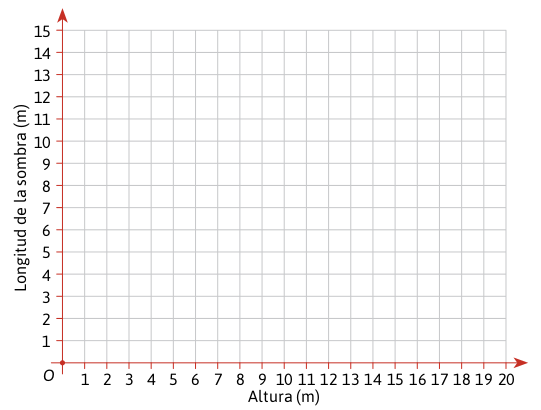
\includegraphics[width=0.65\linewidth]{../images/plano_sombras}
    \captionof{figure}{}
    \label{fig:plano_sombras}
\end{figure}

